
\documentclass{article}
\usepackage{fontenc}
\usepackage[english]{babel}
\usepackage[latin1]{inputenc}
\usepackage{babel}
\usepackage{indentfirst} %auto-indent first paragraphs in sections
\usepackage{verbatim}
\usepackage{url}
\usepackage{fancyhdr} % Required for custom headers
\usepackage{lastpage} % Required to determine the last page for the footer
\usepackage{extramarks} % Required for headers and footers
\usepackage{graphicx} % Required to insert images
\usepackage{subfigure} %for horizontally placed pictures
\usepackage{hyperref} %to make table of contents clickable
\hypersetup{
	colorlinks,
	citecolor=black,
	filecolor=black,
	linkcolor=black,
	urlcolor=black
	}

\usepackage{multirow}

% Margins
\topmargin=-0.45in
\evensidemargin=0in
\oddsidemargin=0in
\textwidth=6.5in
\textheight=9.0in
\headsep=0.25in 
\linespread{1.1} % Line spacing

% Set up the header and footer
\pagestyle{fancy}
\lhead{\myAuthorName} % Top left header
\chead{\myTitle} % Top right header
%\rhead{\myDate}
\rhead{\today}
\lfoot{} % Bottom left footer
\cfoot{} % Bottom center footer
\rfoot{Page\ \thepage\ of\ \pageref{LastPage}} % Bottom right footer
\renewcommand\headrulewidth{0.4pt} % Size of the header rule
\renewcommand\footrulewidth{0.4pt} % Size of the footer rule

\newcommand{\myTitle}{Cluster Matching Algorithms Documentation}
\newcommand{\myAuthorName}{David Caratelli, Ariana Hackenburg}
%\newcommand{\myDate}{January, 2013}
%----------------------------------------------------------------------------------------


\title{\myTitle}
\author{\myAuthorName}
\date{\today}


\begin{document}
\maketitle

\newpage

\tableofcontents

\newpage


%%%%%%%%%%%%%%%%%%%%%%%%%%%%%%%%%%%%%%%%%%
\section{Introduction}
In order to fully reconstruct 3D objects from 2D signals in (wire, time) coordinates information from multiple wire-planes in a TPC must be combined.
2D clusters from multiple planes can be associated together to create a 3D shower. Any particle that deposits energy in the TPC will leave a signature
on all 3 planes. Correctly identifying the deposited energy on different planes associated to the same particle is necessary to reconstruct 3D objects.
We call this process {\bf matching}.\\
Matching is a stage of shower reconstruction that follows cluster merging on individual planes and serves as input to the final shower reconstruction.
Once clusters from two or more planes are associated together a 3D shower can be reconstructed.\\
A number of matching algorithms have been developed to perform this task. Each matching algorithm, given 2 or more clusters on different planes,
returns a score that indicates the compatibility (or matching score) between those clusters. Several algorithms can be used in conjunction. A manager
then handles how to use the information provided by the algorithm. In this document we will describe the matching algorithms currently available.

\newpage

\section{Matching Algorithms}
\subsection{CFAlgoStartPointMatch}
This algorithm is useful only when three clusters on three different planes are given as input. The algorithm calculates a match score only by
looking at the start point of the clusters on the three different planes. For each pair of planes the (Y,Z) intersection point of the wires on 
which the start points of the clusters are found is calculated. This way, three different (Y,Z) intersection points are calculated. A score inversely
proportional to the area of the triangle bound by these three points is returned. A better agreement between the start wires of the clusters leads
to closer (Y,Z) intersection points, which means a smaller area. If for any pair of clusters no intersection point is found, a negative score is returned.
Fig.~\ref{fig:StartPointMatch} illustrates how this algorithm works.
\begin{figure}[!h]
\begin{center}
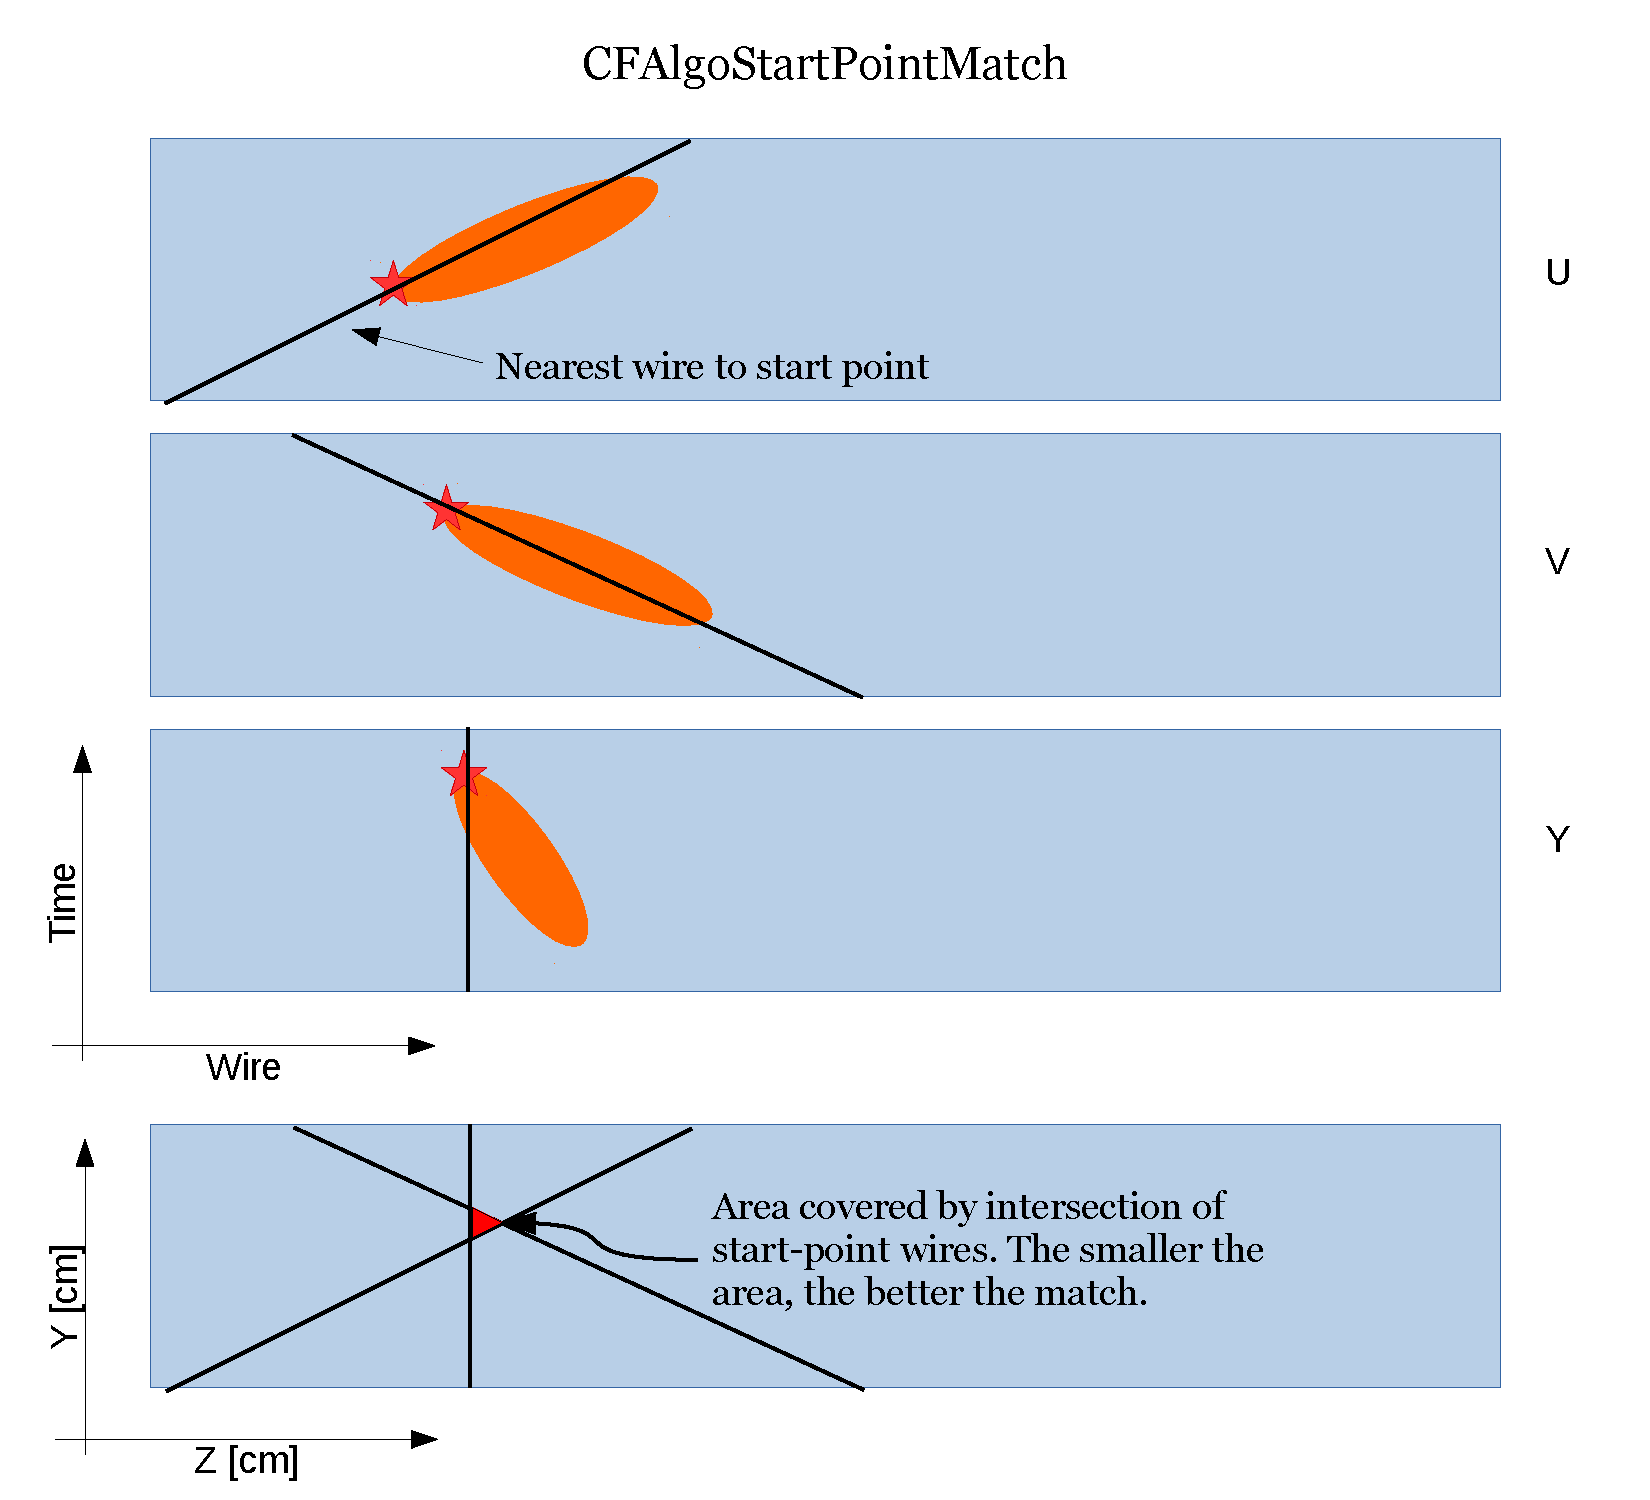
\includegraphics[width=110mm]{Figures/MatchAglo_CFAlgoStartPointMatch_Description.pdf}
\end{center}
\caption{\textit{Illustration highliting how CFAlgoStartPointMatch uses the start wire of three clusters to calculate a measure of the compatibility
between the three clusters}}
\label{fig:StartPointMatch}
\end{figure}

\newpage

\subsection{CFAlgoWireOverlap}
This algorithm finds a rough measure of the area ovelapped by multiple clusters. For each cluster a band of wires determines a polygon on the (Y,Z) plane 
of the TPC. The intersection between different wire-bands on different planes is the wire-overlap that is used to determine the match score for this 
algorithm. Correctly matched clusters should have a large overlap.
Fig.~\ref{fig:WireOverlap} illustrates how this algorithm works.
\begin{figure}[!h]
\begin{center}
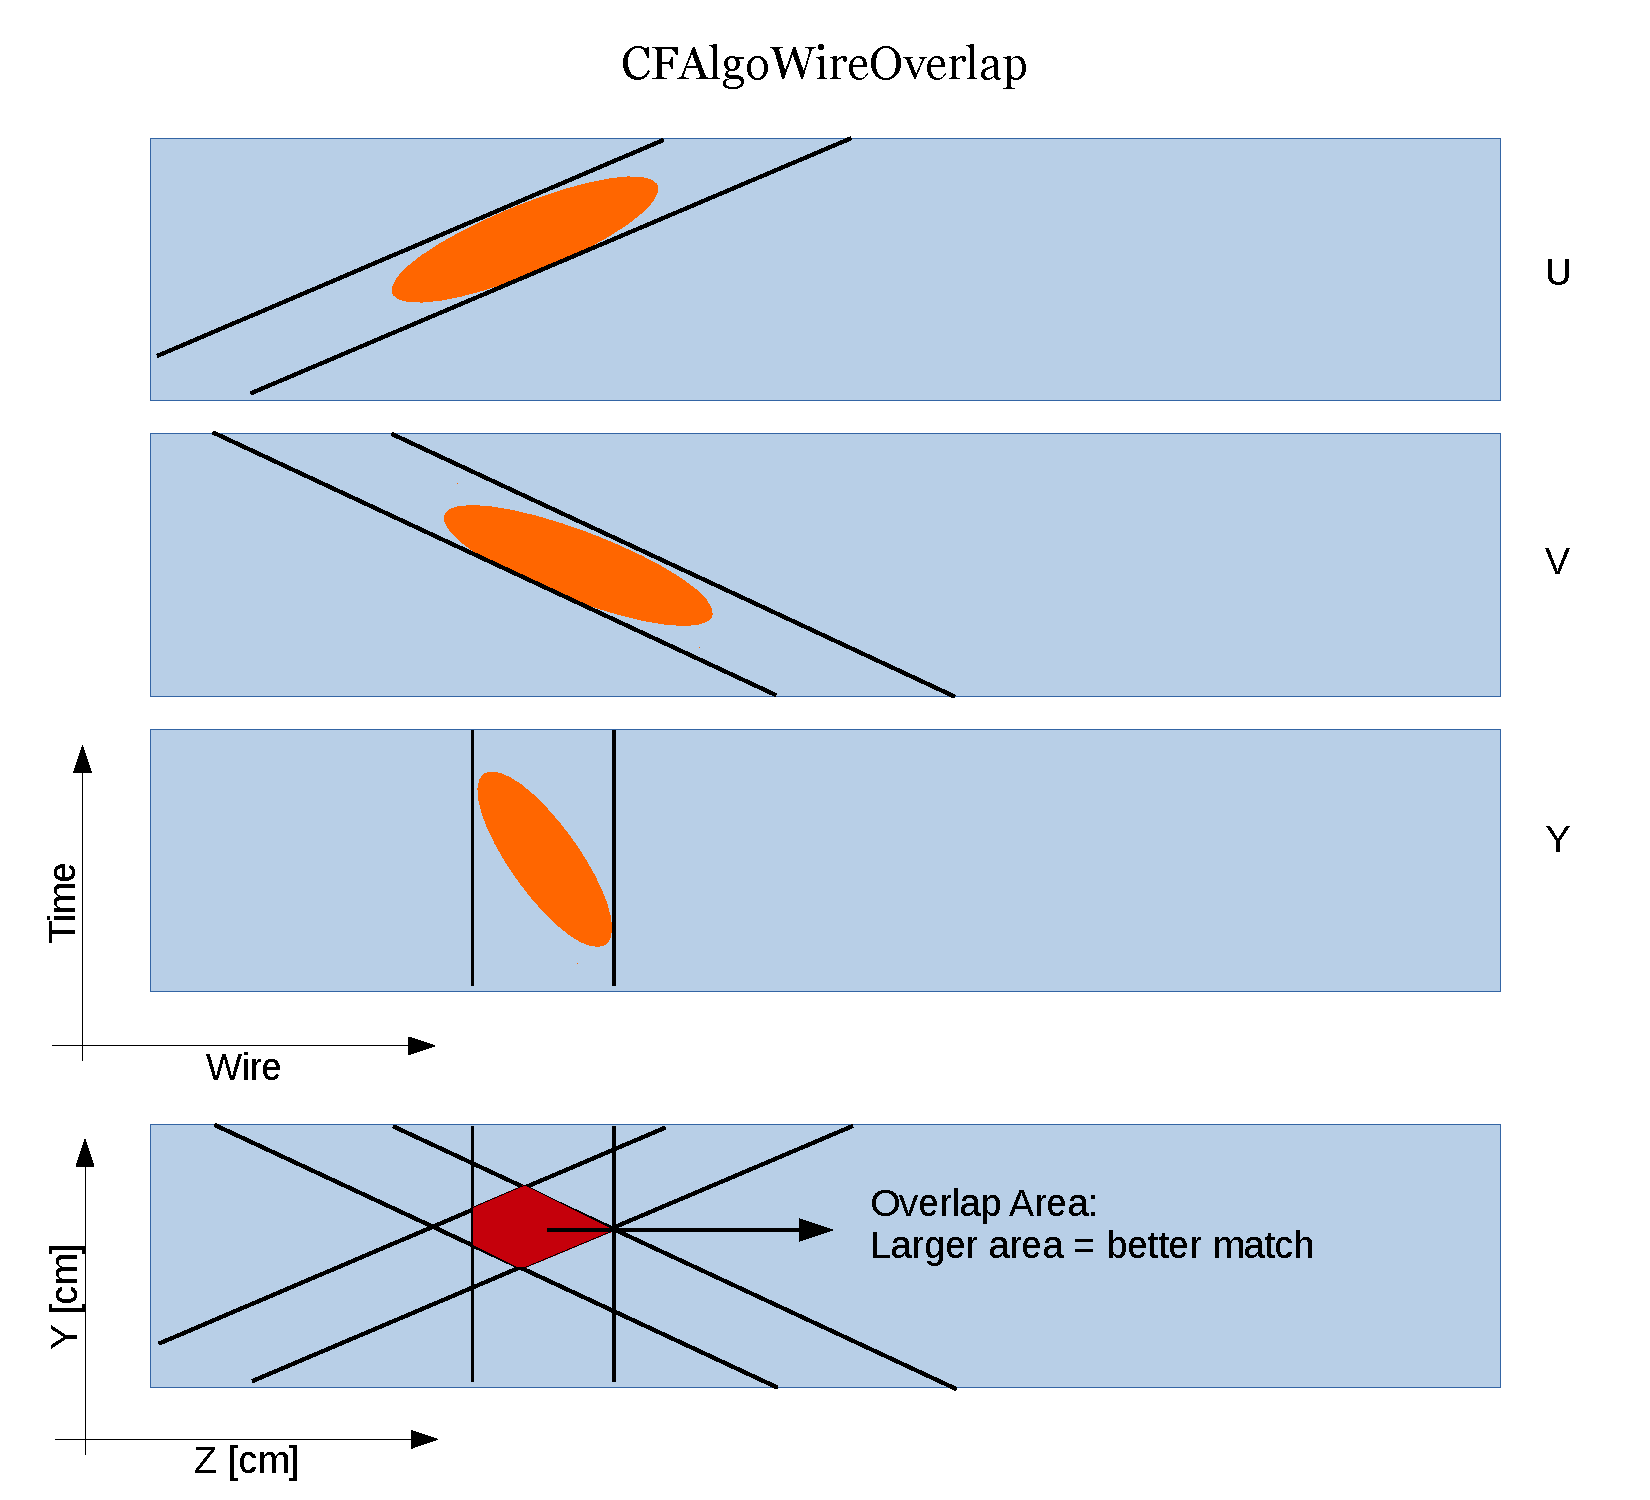
\includegraphics[width=110mm]{Figures/MatchAglo_CFAlgoWireOverlap_Description.pdf}
\end{center}
\caption{\textit{Illustration highliting how CFAlgoWireOverlap uses overlapping wire-bands of clusters on different planes to calcualte a match score.}}
\label{fig:VolumeOverlap}
\end{figure}

\newpage

\subsection{CFAlgoVolumeOverlap}
This algorithm finds a rough measure of the TPC volume overlapped by multiple clusters on different planes. A score proportional to the overlapping volume
is returned as the match score. The overlapping volume is calculated as follows:\\
- An overlapping time window between all clusters is found. This is then converted in cm (the overlap in X)\\
- Each cluster's start and end wire are used to determine a band of wires defining the cluster's projection in (Y,Z) space. The intersection polygon common
to all wire-bands determines the intersection area in (Y,Z) space.\\
- Finally, the intersection area in (Y,Z) is multiplied by the overlap region in X to get an overlap volume. This value is returned as the match score.
Fig.~\ref{fig:VolumeOverlap} illustrates how this algorithm works.
\begin{figure}[!h]
\begin{center}
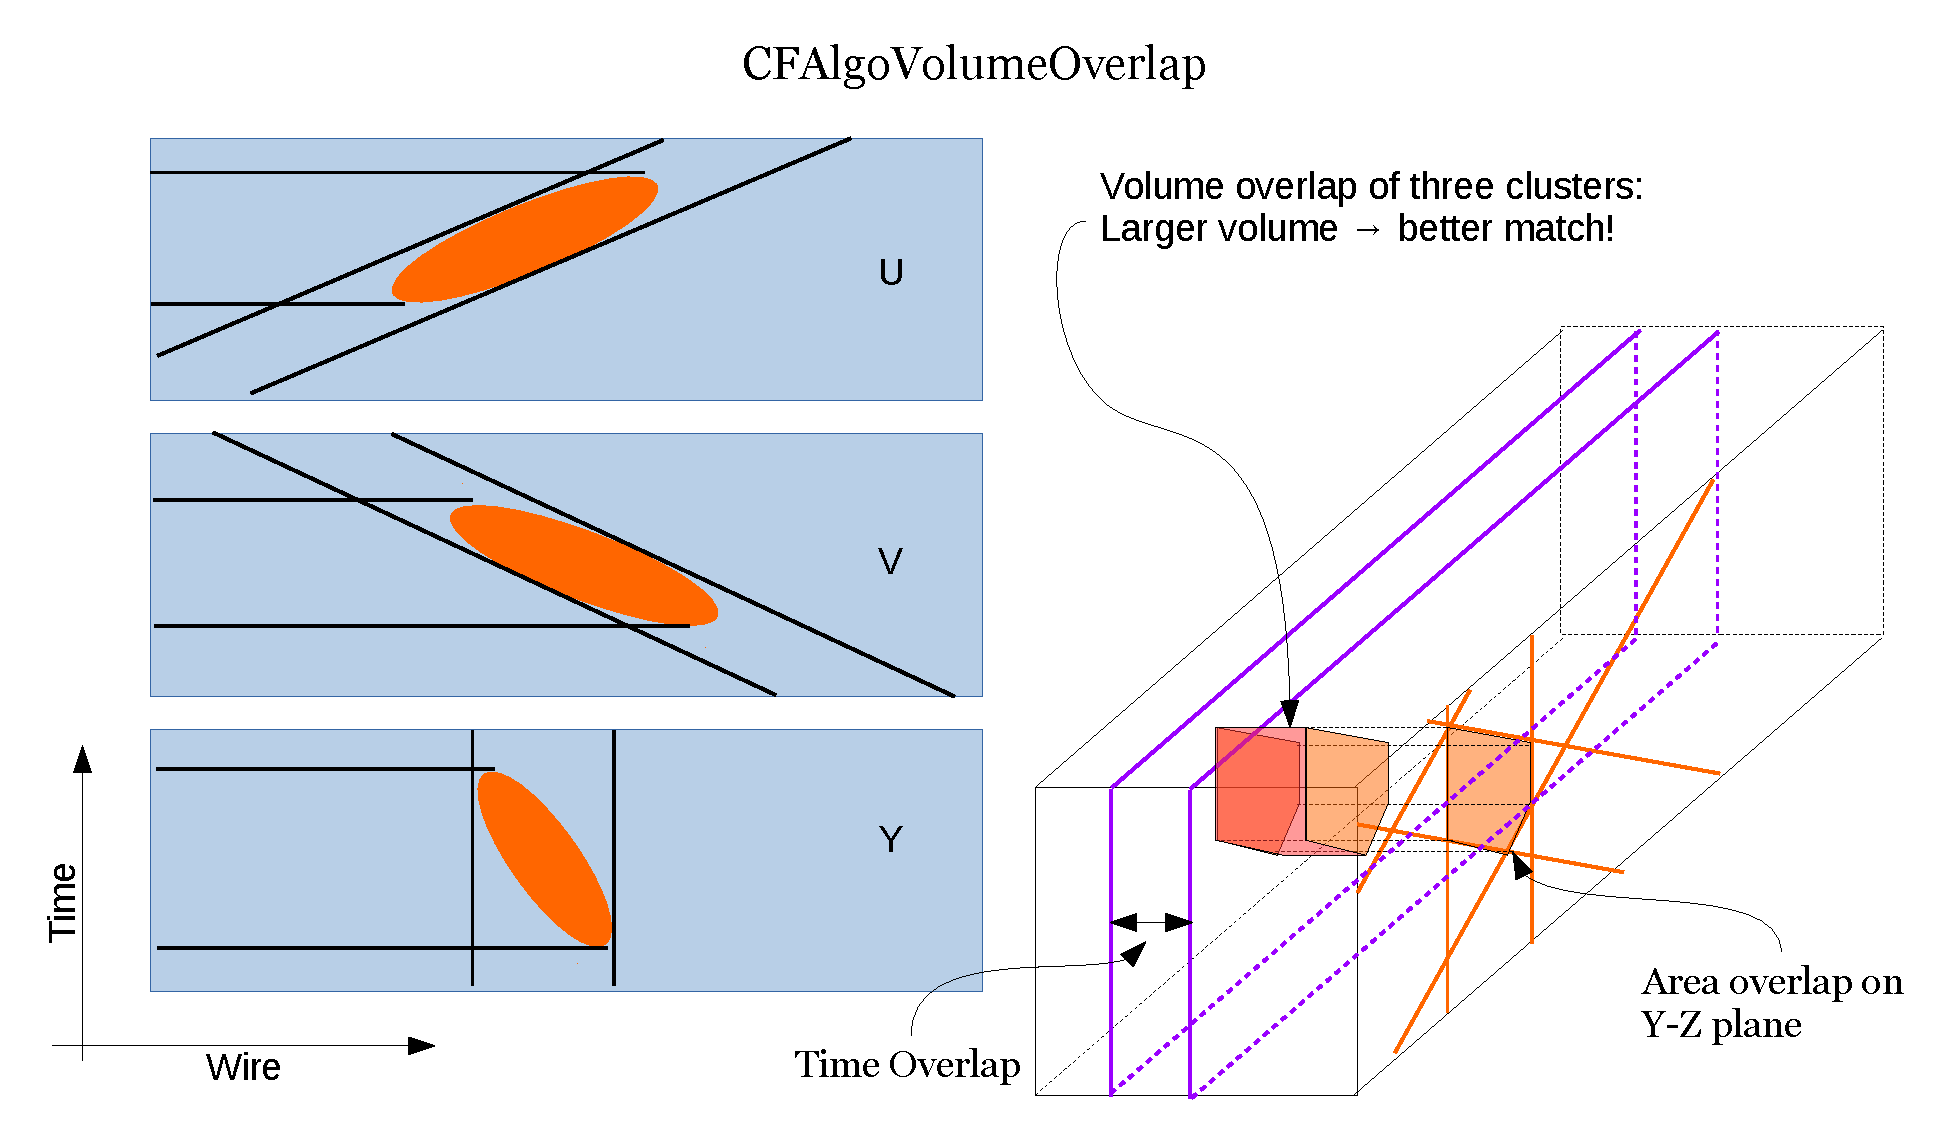
\includegraphics[width=110mm]{Figures/MatchAglo_CFAlgoVolumeOverlap_Description.pdf}
\end{center}
\caption{\textit{Illustration highliting how CFAlgoVolumeOverlap uses the time and wire intersections across planes to calculate an overlapping volume
common to all clusters.}}
\label{fig:VolumeOverlap}
\end{figure}

\newpage

\subsection{CFAlgoChargeDistrib}
This algorithm looks at the charge distribution in time for multiple clusters. Clusters that truly belong to the same particle should see similar charge
distributions in time. This algorithm computes a convolution (of sorts) of the time-distribution of the charge in clusters on different planes. The larger
this convolution, the larger the score returned by the algorithm.\\
For each cluster, the distribution in time of the charge collected in the hits belonging to the clusters is scaled to a unit vector so that the charge from
the hit with the smallest time is at 0 and that from the hit with the largest time is at 1. The charge distributions are then compared. The intersection
of the two distributions is calculated. This intersection is a measure of the convolution of the charge distributions on the various clusters and it is
used as the match score for this algorithm. Fig.~\ref{fig:ChargeDistrib} illustrates how this convolution is calculated.
\begin{figure}[!h]
\begin{center}
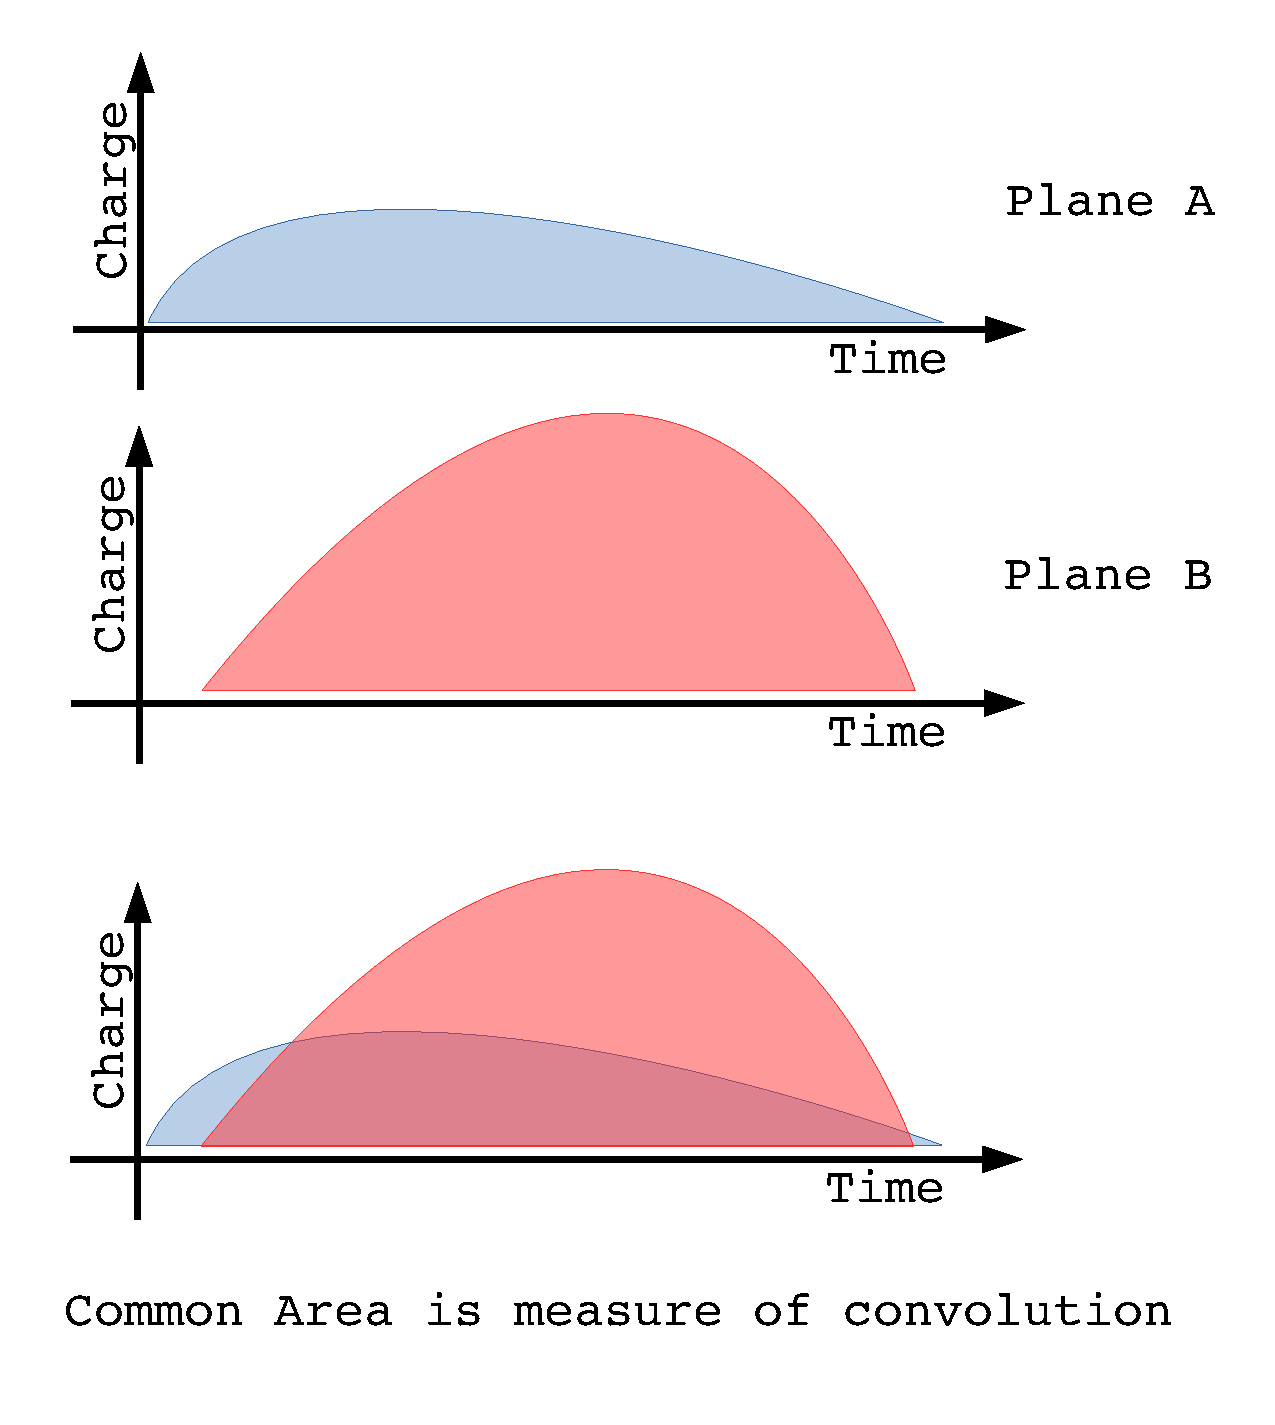
\includegraphics[width=110mm]{Figures/MatchAglo_CFAlgoChargeDistrib_Description.pdf}
\end{center}
\caption{\textit{Illustration highliting how CFAlgoChargeDistrib calculates a match score by comparing the time-distribution of charge on each cluster.}}
\label{fig:ChargeDistrib}
\end{figure}

\newpage

\subsection{CFAlgoQRatio}
This algorithm compares the ratio of charge in the clusters considered. At first, the cluster with the largest charge is found. The charge for this cluster
is denoted as $Q_{{\rm max}}$. A charge ratio is found by calculating:
\begin{equation}
 \sum_{i=0}^{{\rm N_{clusters}}} \frac{Q_i}{Q_{{\rm max}}}
\end{equation}
If this ratio is larger than a certain cut value, the ratio is returned as the score. Otherwise, the return is -1.

\newpage

\subsection{CFAlgoStartPointCompat}
This algorithm works only when clusters on all 3 planes are provided. For every pair of clusters, the intersection in (Y,Z) coordinates of the start-point
wires on those clusters is found. This (Y,Z) point is then projected back to the plane of the 3rd cluster and the wire on the 3rd plane closest to this point
is found. This is the reconstructed start wire on the 3rd plane. If this reconstructed start wire is in-between the start and end wires of the cluster
on the third plane, the closer of the two to the reconstructed start wire is chosen. The inverse of the distance between these two is taken as the matching
score. For a group of 3 clusters this calculation can be repeated for 3 different combinations. The highest score across all three combinations is finally
returned by the algorithm. Fig.~\ref{fig:StartPointCompat} illustrates how CFAlgoStartPointCompat works..
\begin{figure}[!h]
\begin{center}
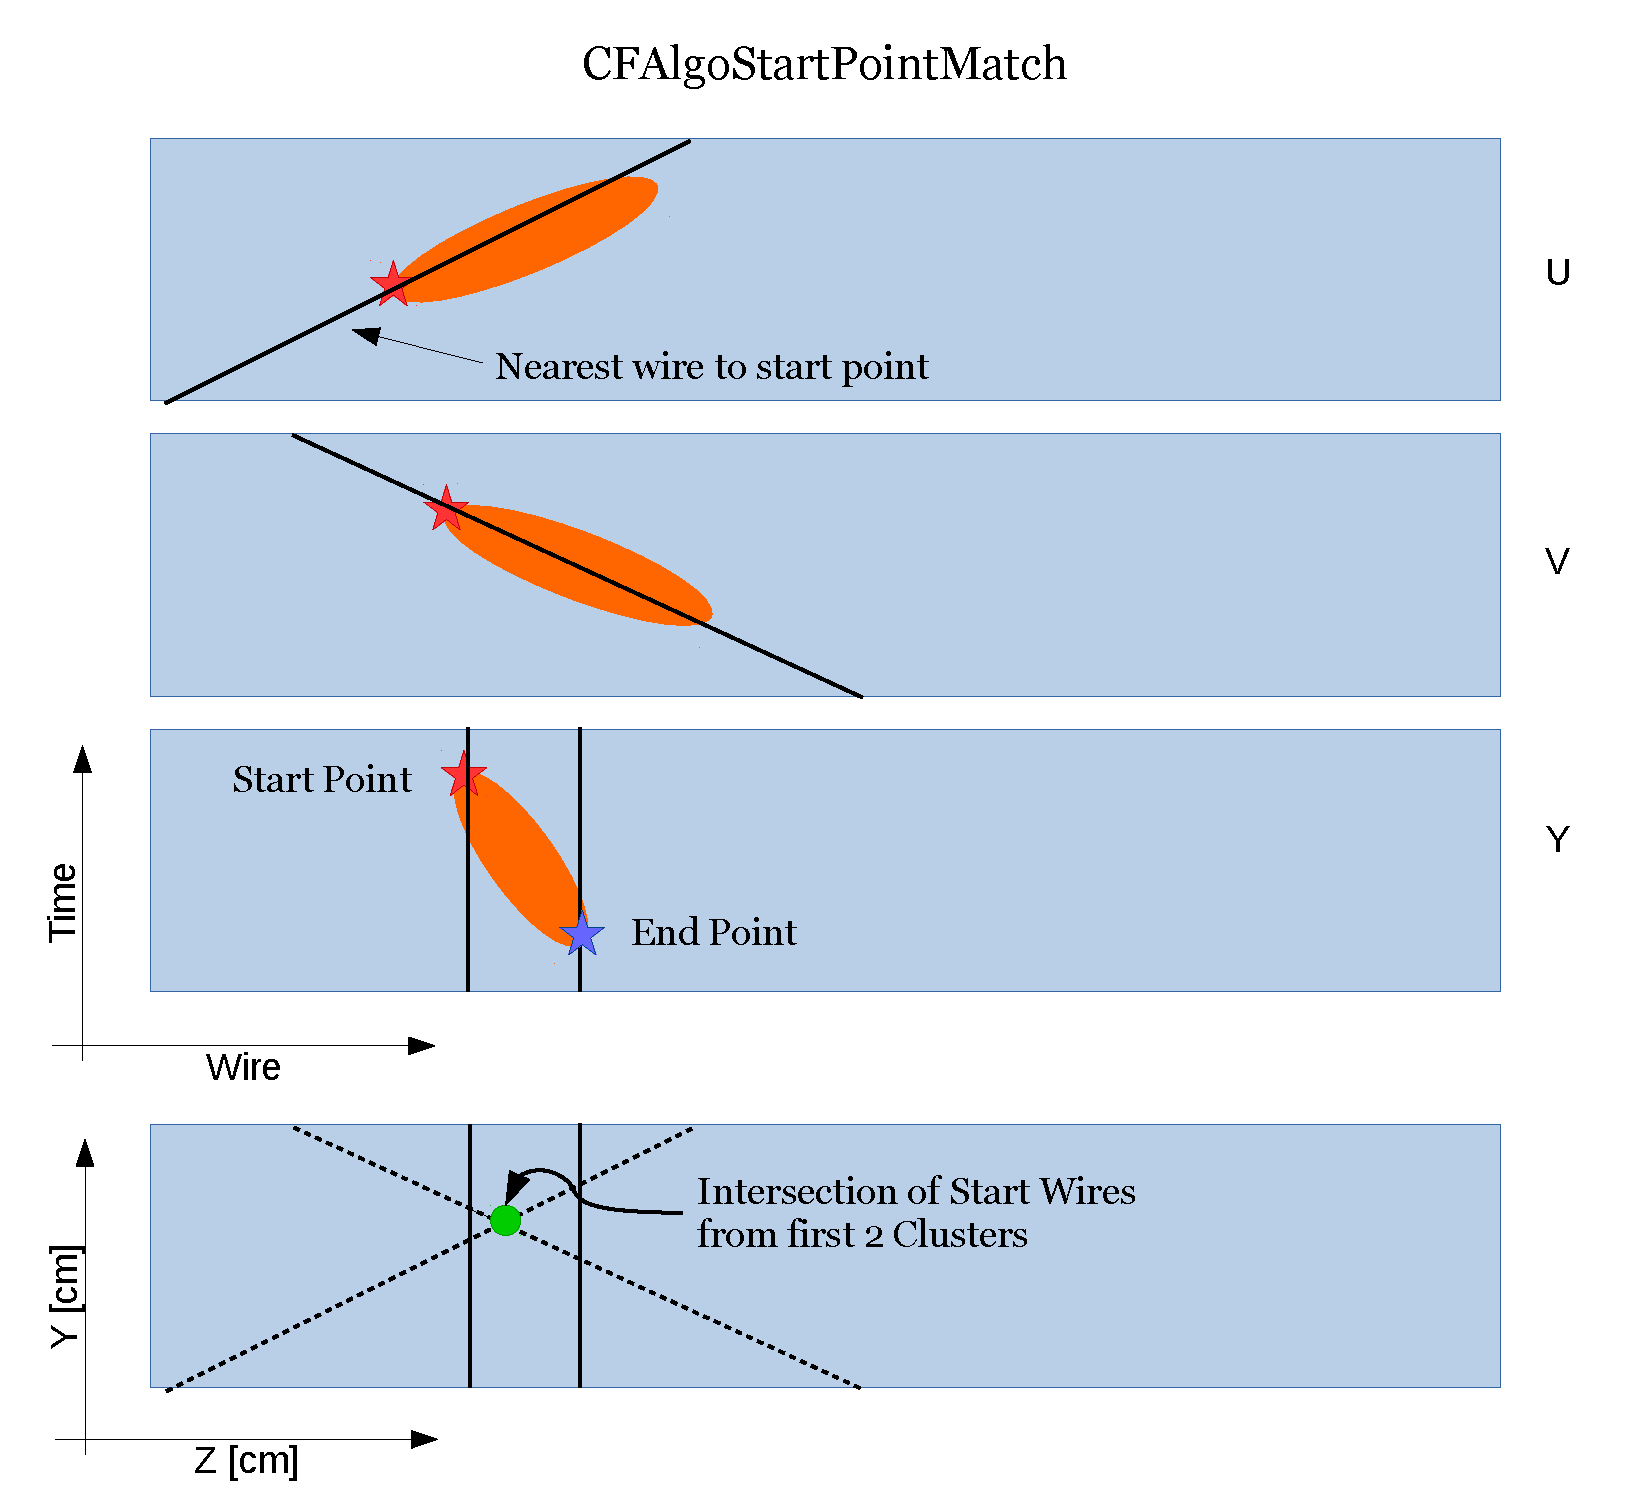
\includegraphics[width=110mm]{Figures/MatchAglo_CFAlgoStartPointCompat_Description.pdf}
\end{center}
\caption{\textit{Illustration highliting how CFAlgoStartPointCompat calculates a match score by checking the compatibility of the start point
reconstructed using two planes, with the cluster information on the 3rd plane..}}
\label{fig:StartPointCompat.}
\end{figure}


\end{document}

